\documentclass[../main.tex]{subfiles}
\begin{document}

    Ma na celu \textbf{wypełnienie luki między obiektami dziedziny aplikacyjnej a komponentami} wybranymi na etapie projektowania systemu.


    \begin{figure}[h]
        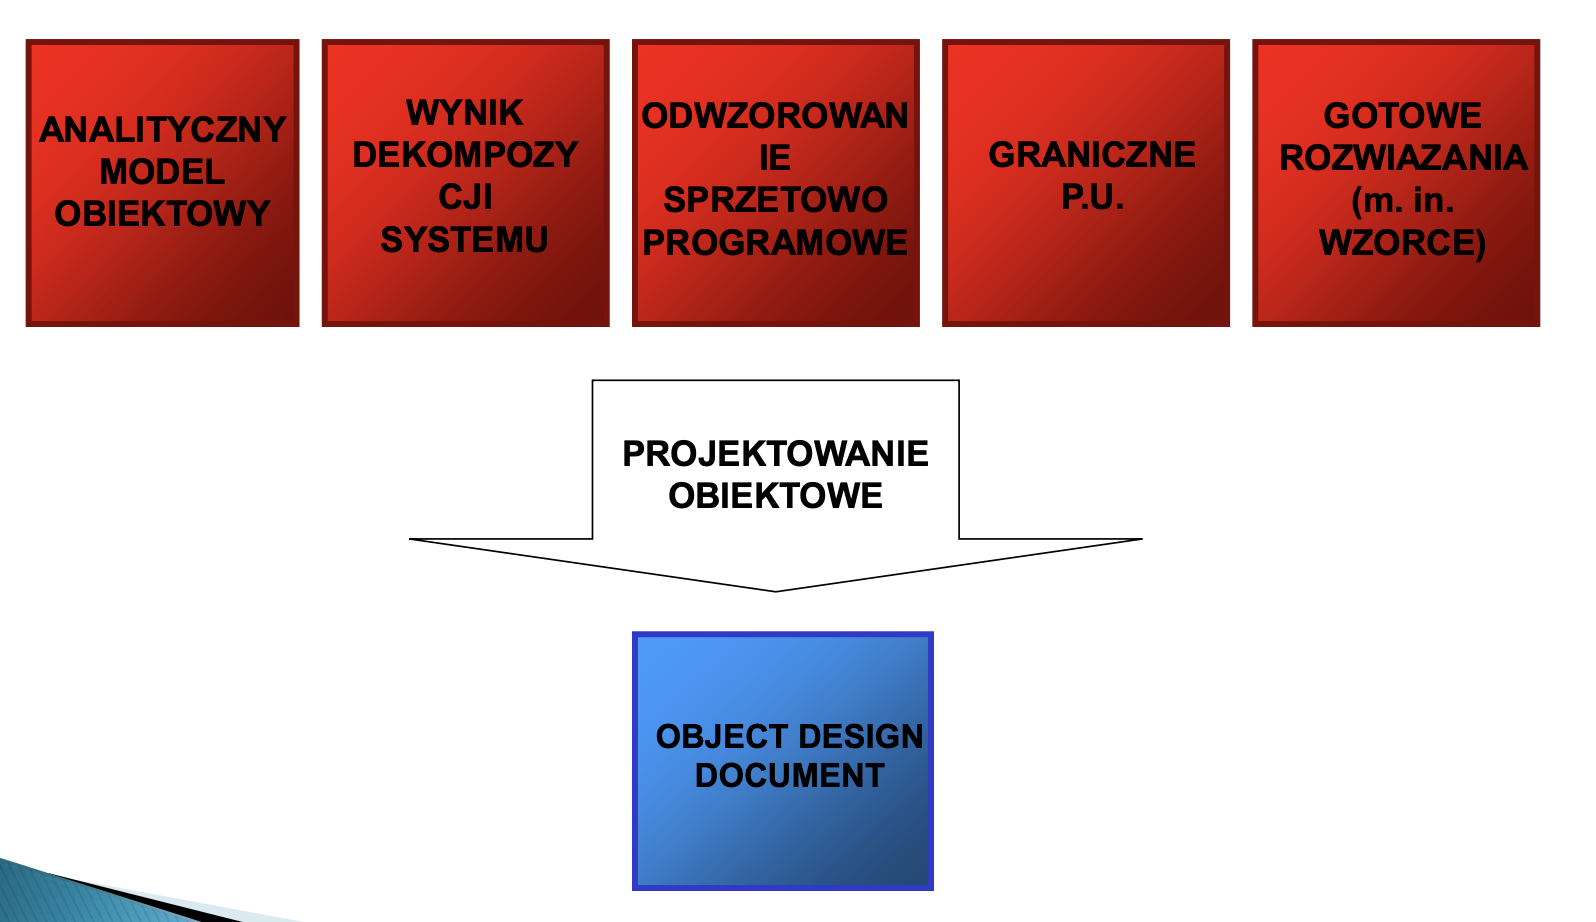
\includegraphics[width=\linewidth]{projektowanie_obiektow.png}
    \end{figure}

    \textbf{Etapy projektowania obiektów}
    \begin{itemize}
        \item wykorzystanie gotowych rozwiązań, którymi są zarówno
        gotowe produkty (komponenty) jak i wzorce projektowe;
        \item specyfikowanie usług;
        \item restrukturyzacja modelu obiektowego;
        \item optymalizacja modelu obiektowego;
    \end{itemize}

    \begin{figure}[H]
        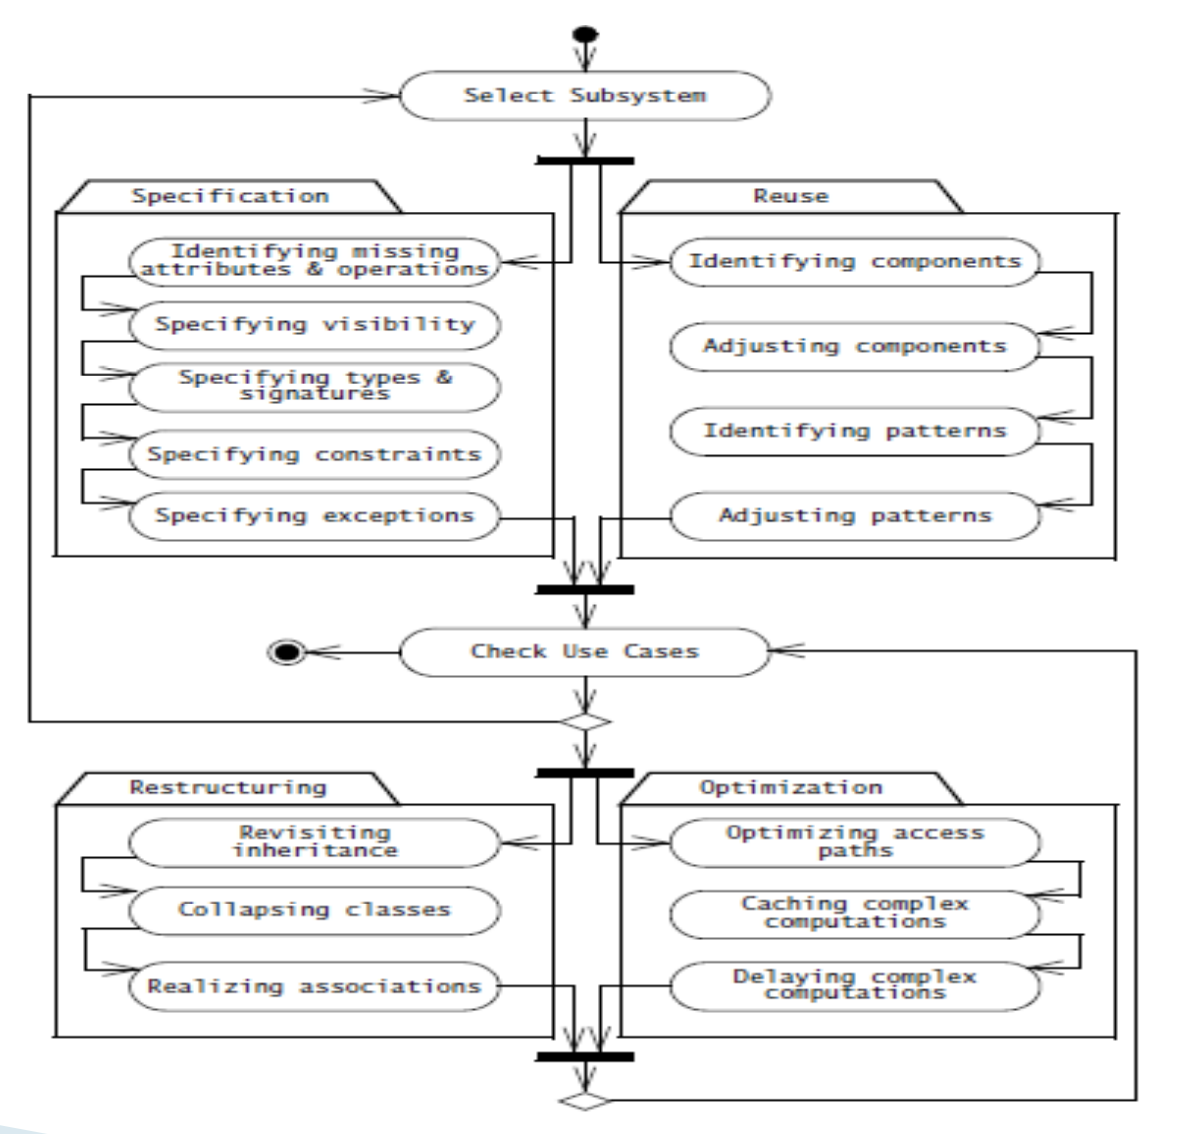
\includegraphics[width=\linewidth]{subsystem.png}
    \end{figure}

    Koncepcje wielokrotnego wykorzystywania gotowych rozwiązań:
    \begin{itemize}
        \item \textbf{obiekty aplikacyjne} - reprezentują koncepcje problemowe związane z tworzonym systemem.
        \item \textbf{obiekty realizacyjne} - reprezentują komponenty nie mające odpowiedników w
        dziedzinie aplikacyjnej, na przykład bazy danych czy obiekty interfejsu użytkownika.
        \item \textbf{dziedziczenie implementacyjne} - ma miejsce jeśli sięgamy po dziedziczenie z zamiarem wykorzystania
        gotowego kodu, mimo różnic koncepcyjnych pomiędzy powiązanymi klasami.
        \item \textbf{dziedziczenie specyfikacyjne} - ma odzwierciedlenie w taksonomii klas (reprezentuje podtypowanie).
        \item \textbf{delegowanie implementacji} - zamiast implementować set jako nadpisywanie metod hashtable, implementujemy go jako set korzystajacy z instancji hashtable z własnymi metodami.
        Rozwiązuje problemy dziedziczenia implementacyjnego: rozszerzalność, podtypowanie.
        \item \textbf{zasada zastępowania Liskov} - \textit{'Jeśli obiekt klasy S może stać się substytutem obiektu klasy T w
        dowolnym miejscu kodu, w którym oczekiwany jest obiekt klasy T, to klasa S jest podtypem klasy T.'}
        \item \textbf{wzorce projektowe} (obiektowe);
    \end{itemize}



    \subsection{Wzorce projektowe - poziom interakcji między klasami}
    \textbf{Wzorzec opisuje problem, który powtarza się wielokrotnie w danym środowisku, oraz podaje istotę
    jego rozwiązania.}

    \begin{itemize}
        \item Czy typowe problemy można rozwiązać w powtarzalny sposób?
        \item Czy te problemy można przedstawić w sposób abstrakcyjny, tak aby były pomocne
        w tworzeniu rozwiązań w róznych konkretnych kontekstach?
    \end{itemize}

    \begin{itemize}
        \item \textbf{Wzorce kreacyjne}
        \begin{itemize}
            \item abstrakcyjne metody tworzenia obiektów,
            \item uniezależnienie systemu od sposobu tworzenia obiektów.
        \end{itemize}
        \item \textbf{Wzorce strukturalne}
        \begin{itemize}
            \item sposób wiązania obiektów w struktury,
            \item właściwe wykorzystanie dziedziczenia i kompozycji.
        \end{itemize}
        \item \textbf{Wzorce behawioralne}
        \begin{itemize}
            \item algorytmy i przydział odpowiedzialności,
            \item opis przepływu kontroli i interakcji.
        \end{itemize}
    \end{itemize}

    \subsection{Koncepcje specyfikowania interfejsów}
    \begin{itemize}
        \item implementator (realize class), ekstender (refine class) i użytkownik (use class) klasy,
        \item typy, sygnatury (wektory/krotki typów parametrów i typu wyniku) i widzialność (public, private, protected, packet),
        \item kontrakty: niezmienniki, warunki wstępne i warunki końcowe,
        \item język OCL (Object Constraint Language) – ograniczenia, zbiory, wielozbiory i ciągi; kwantyfikatory.
    \end{itemize}

    \subsection{Aktywności specyfikowania interfejsów}
    \begin{itemize}
        \item identyfikowanie brakujących atrybutów i operacji;
        \item definiowanie widzialności i sygnatur;
        \item specyfikowanie kontraktów;
        \item dziedziczenie kontraktów;
    \end{itemize}



    \subsection{SOLID}

    \begin{itemize}
        \item \textbf{Single responsibility principle}
        \begin{itemize}
            \item Klasa powinna mieć pojedyńczą odpowiedzialność.
            \item Nigdy nie powinien istnieć więcej niż jeden powód do modyfikacji klasy.
            \item Im mniejsza i bardziej wyspecyfikowana klasa tym łatwiej ją nazwać.
            \item Łatwiejsze wprowadzanie zmian,testowanie i naprawa
        \end{itemize}
        Jak rozpoznać naruszenie SRP?
        \begin{itemize}
            \item Ilość linii kodu ( Class:LOC > 250),
            \item Za dużo zależności, słaba spojność, dużo zagnieżdżeń,
            \item Opis lub nazwa wymaga “i”,
            \item Wymaga skomplikowanych testów,
            \item Modyfikacja może zepsuć inne testy.
        \end{itemize}
        \item \textbf{Open/closed principle}
        \begin{itemize}
            \item klasa powinna być otwarta na rozbudowę, ale zamknięta do jej własnej modyfikacji,
            \item możemy dodawać nowe pola i metody, ale bez zmiany w wewnętrznej strukturze,
            \item zmiana istniejącej struktury może mieć wpływ na inne elementy,
            \item hermetyzacja, dziedziczenie, polimorfizm, delegaty,
            \item unikamy instrukcji warunkowych.
        \end{itemize}
        \item \textbf{Liskov substitution principle}
        \begin{itemize}
            \item 'Jeśli obiekt klasy S może stać się substytutem obiektu klasy T w
            dowolnym miejscu kodu, w którym oczekiwany jest obiekt klasy T, to klasa S jest podtypem klasy T.'
        \end{itemize}
        \item \textbf{Interface segregation principle}
        \begin{itemize}
            \item Kilka konkretnych interfejsów jest lepszych niż jeden ogólny,
            \item Związki między klasami powinny być ograniczone do minimum,
            \item Klient klasy powinien mieć dostep tylko do tyh składowych klasy, których rzeczywiście potrzebuje,
            \item Moduły wysokiego poziomu nie powinny zależeć od modułów niskopoziomowych,
            \item Obie grupy modułów powinny zależeć od abstrakcji.
        \end{itemize}
        \item \textbf{Dependency inversion principle} - zasada odwracania zależności.
        \begin{itemize}
            \item Software powinien zależeć od abstrakcji a nie od konkretyzacji,
            \item 'Hollywood Principle' - don't call us, we'll call you!.
        \end{itemize}
    \end{itemize}


    \subsection{Wybrane wzorce kreacyjne}

    \begin{table}[H]
        \begin{center}
            \begin{tabular}{  p{8cm} c  }
                \toprule
                Wzorzec & Schemat \\

                \cmidrule(r){1-1}\cmidrule(l){2-2}
                \textbf{Singleton}
                \begin{itemize}
                    \item Zapewnienie, że \textbf{klasa posiada jedną instancję} wewnątrz całej aplikacji
                    \item Stworzenie punktu dostępowego do tej instancji
                \end{itemize}
                &
                \raisebox{-\totalheight}{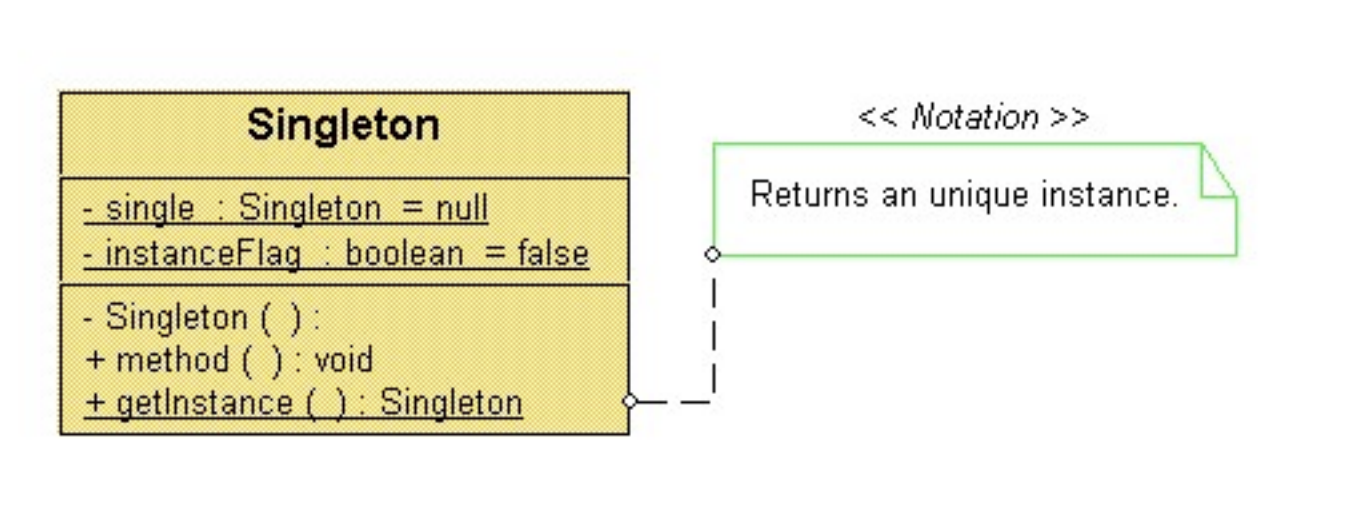
\includegraphics[width=0.5\textwidth, height=60mm]{singleton.png}}
                \\

                \cmidrule(r){1-1}\cmidrule(l){2-2}
                \textbf{Factory method}
                \begin{itemize}
                    \item Zdefiniowanie \textbf{interfejsu do tworzenia obiektów}
                    \item Umożliwienie przekazania odpowiedzialności za tworzenie obiektów do podklas
                    \item Umożliwienie wyboru klasy i konstruktora użytego do utworzenia obiektu
                \end{itemize}
                &
                \raisebox{-\totalheight}{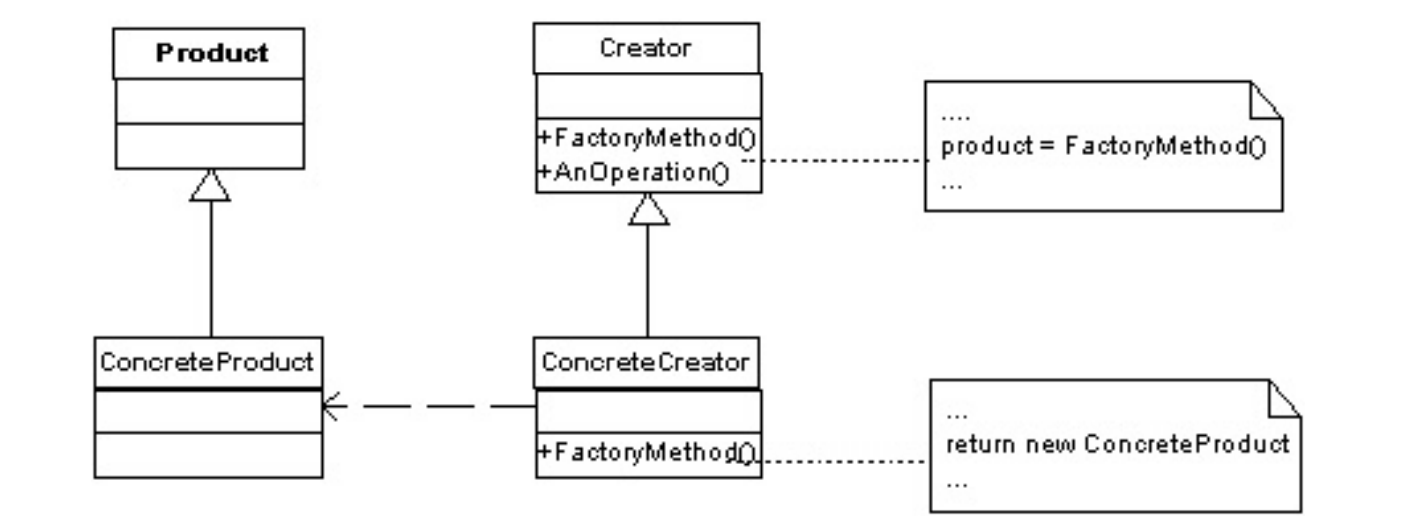
\includegraphics[width=0.5\textwidth, height=60mm]{fac-met.png}}
                \\

                \cmidrule(r){1-1}\cmidrule(l){2-2}
                \textbf{Builder}
                \begin{itemize}
                    \item \textbf{Odseparowanie sposobu reprezentacji i metody konstrukcji} złożonych struktur obiektowych
                    \item Wykorzystanie jednego mechanizmu konstrukcyjnego do tworzenia struktur o różnej reprezentacji
                \end{itemize}
                &
                \raisebox{-\totalheight}{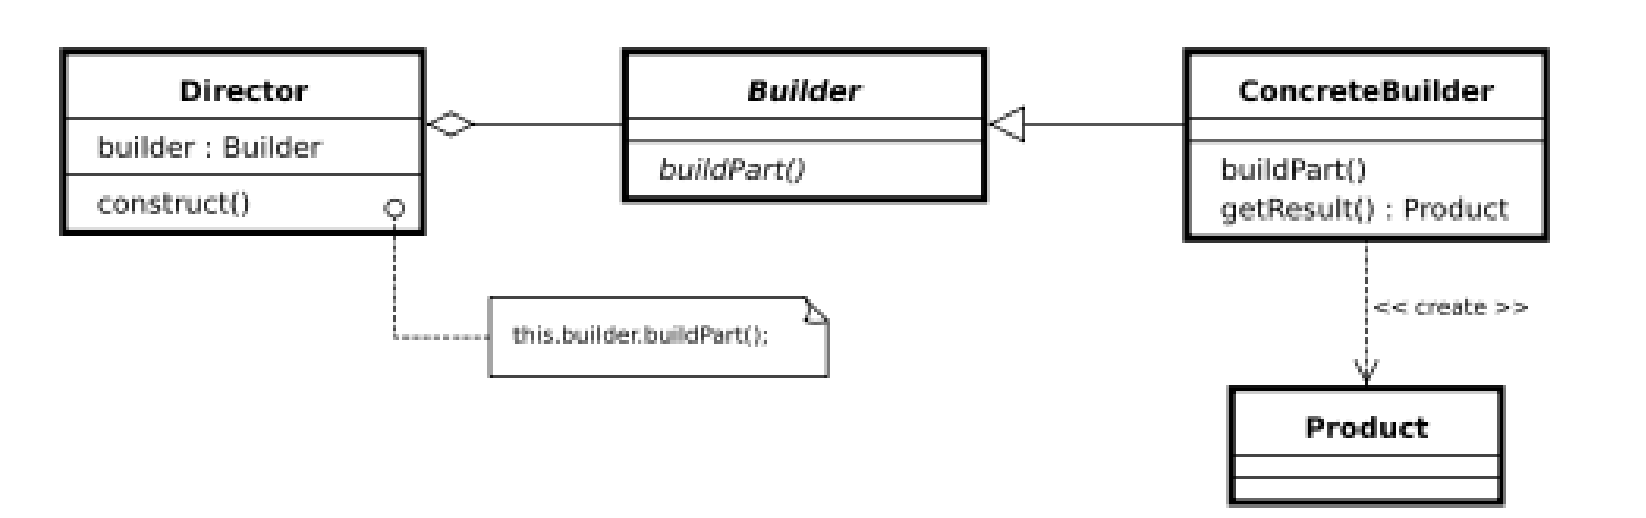
\includegraphics[width=0.5\textwidth, height=60mm]{builder.png}}
                \\


                \bottomrule
            \end{tabular}
        \end{center}
    \end{table}


    \subsection{Wybrane wzorce strukturalne}

    \begin{table}[H]
        \begin{center}
            \begin{tabular}{  p{8cm} c  }
                \toprule
                Wzorzec & Schemat \\

                \cmidrule(r){1-1}\cmidrule(l){2-2}
                \textbf{Adapter}
                \begin{itemize}
                    \item Umożliwia \textbf{współpracę obiektów o niezgodnych typach}
                    \item Tłumaczy protokoły obiektowe
                \end{itemize}
                &
                \raisebox{-\totalheight}{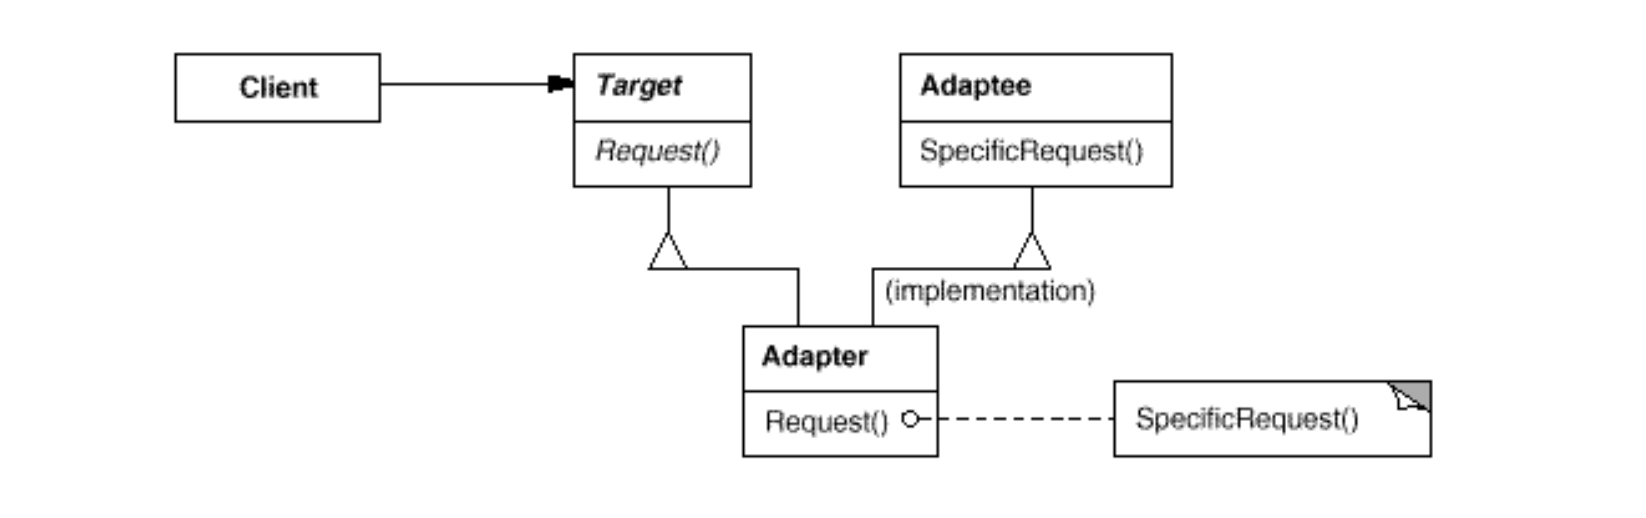
\includegraphics[width=0.5\textwidth, height=60mm]{adapter.png}}
                \\

                \cmidrule(r){1-1}\cmidrule(l){2-2}

                \textbf{Proxy}
                \begin{itemize}
                    \item Dostarcza \textbf{zamiennik obiektu} w celu jego kontroli i ochrony
                    \item Przezroczyste odsuniecie inicjalizacji obiektu w czasie
                \end{itemize}
                &
                \raisebox{-\totalheight}{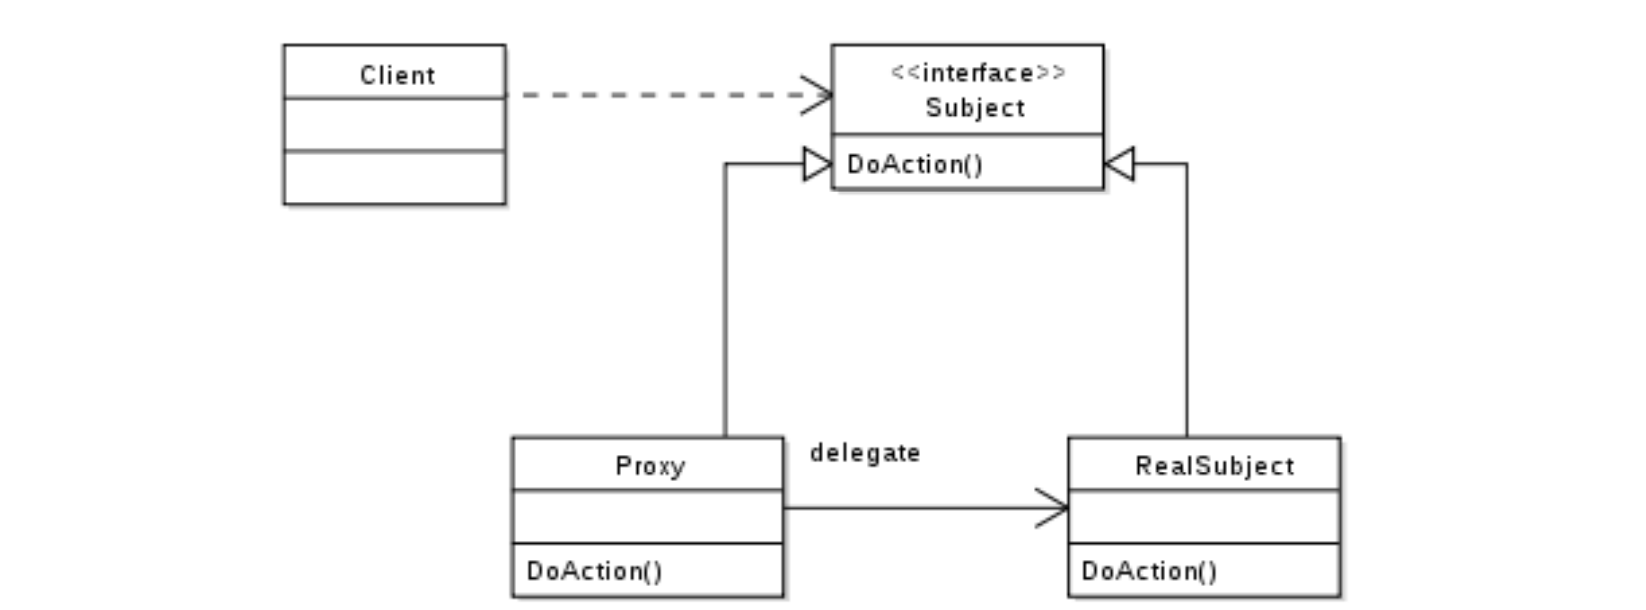
\includegraphics[width=0.5\textwidth, height=60mm]{proxy.png}}
                \\

                \cmidrule(r){1-1}\cmidrule(l){2-2}
                \textbf{Fasada}
                \begin{itemize}
                    \item Dostarczenie \textbf{jednorodnego interfejsu wyższego poziomu} do zbioru różnych interfejsów w systemie
                    \item Ukrycie złożoności podsystemów przed klientem
                \end{itemize}
                &
                \raisebox{-\totalheight}{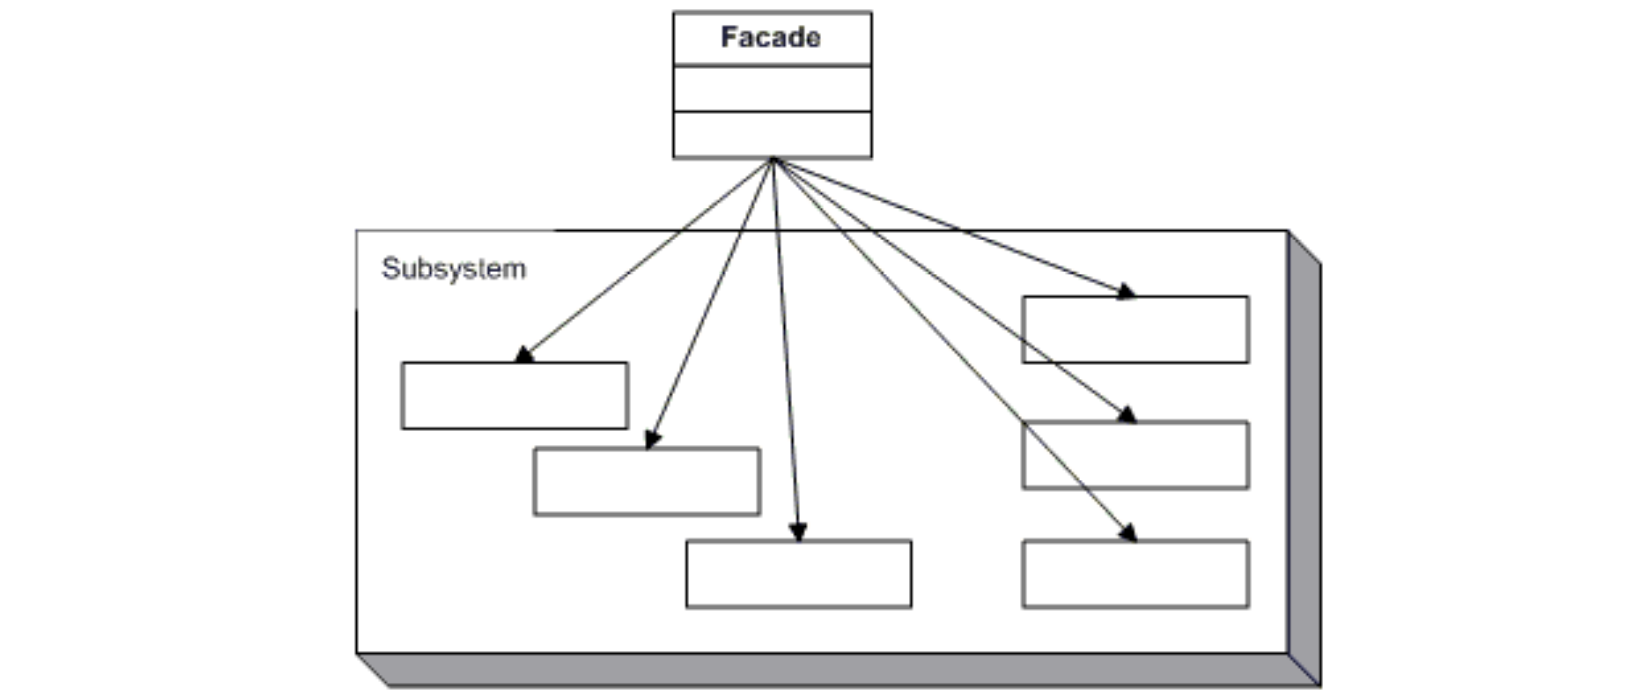
\includegraphics[width=0.5\textwidth, height=60mm]{fasada.png}}
                \\

                \bottomrule
            \end{tabular}
        \end{center}
    \end{table}


    \subsection{Wybrane wzorce behawioralne}

    \begin{table}[H]
        \begin{center}
            \begin{tabular}{  p{8cm} c  }
                \toprule
                Wzorzec & Schemat \\

                \cmidrule(r){1-1}\cmidrule(l){2-2}
                \textbf{Obserwator}
                \begin{itemize}
                    \item Tworzy \textbf{zależność typu jeden-wiele} pomiędzy obiektami
                    \item \textbf{Informacja o zmianie} stanu wyróżnionego obiektu jest \textbf{przekazywana wszystkim pozostałym obiektom}
                \end{itemize}
                &
                \raisebox{-\totalheight}{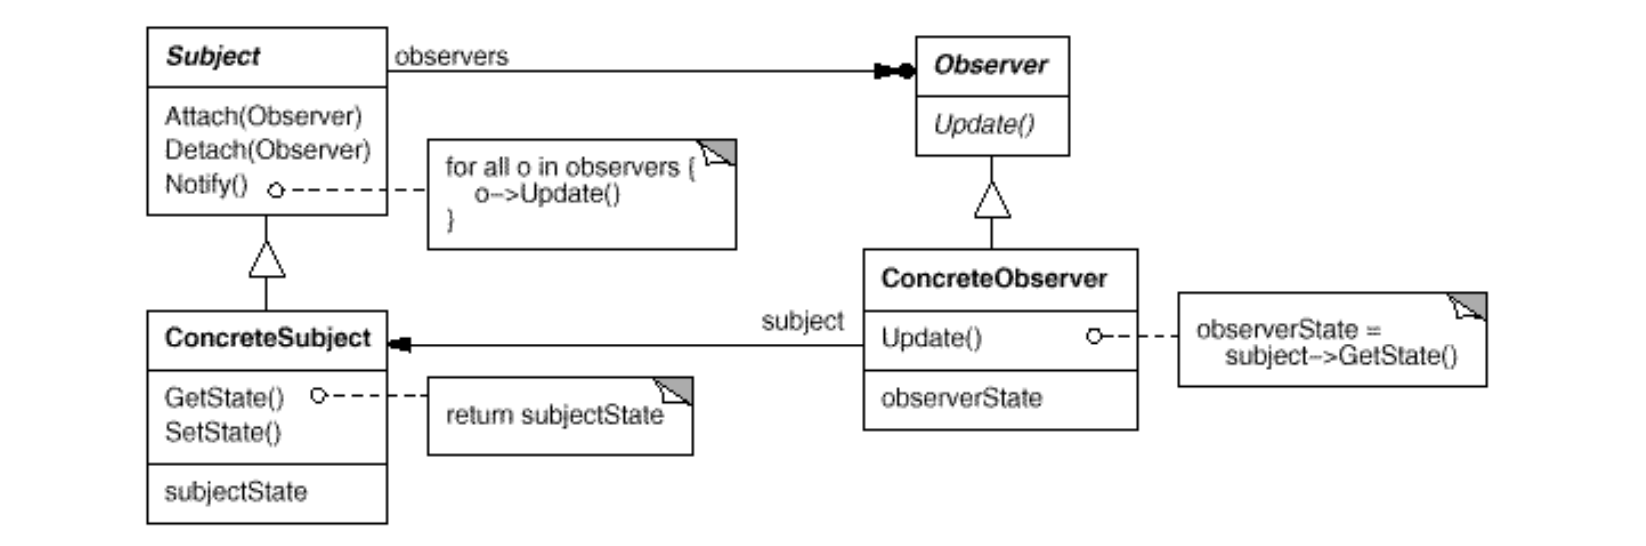
\includegraphics[width=0.5\textwidth, height=60mm]{obserwator.png}}
                \\

                \cmidrule(r){1-1}\cmidrule(l){2-2}
                \textbf{Command}
                \begin{itemize}
                    \item \textbf{Hermetyzacja poleceń} do wykonania w postaci obiektów
                    \item Umożliwienie \textbf{parametryzacji klientów} obiektami poleceń
                    \item Wsparcie dla \textbf{poleceń odwracalnych}
                \end{itemize}
                &
                \raisebox{-\totalheight}{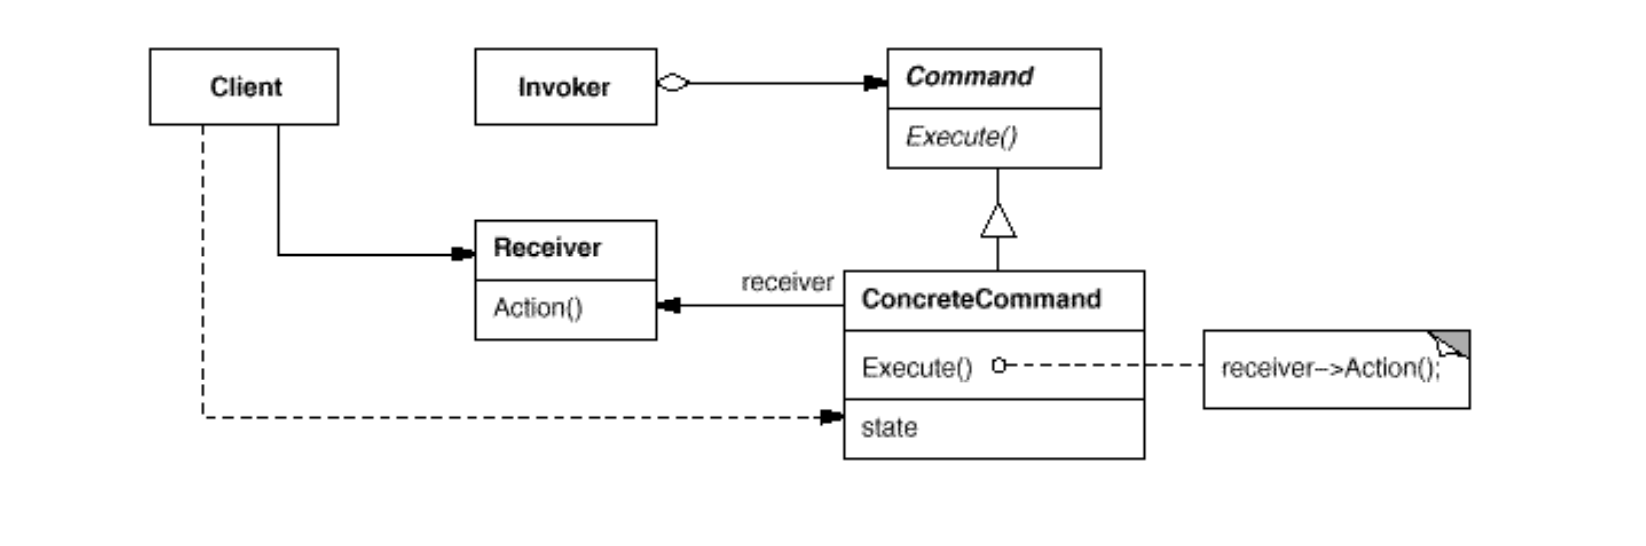
\includegraphics[width=0.5\textwidth, height=60mm]{command.png}}
                \\

                \cmidrule(r){1-1}\cmidrule(l){2-2}
                \textbf{Chain of responsibility}
                \begin{itemize}
                    \item \textbf{Usunięcie powiązania pomiędzy nadawcą i odbiorcą} żądania
                    \item Umożliwienie wielu obiektom obsługi żądania
                \end{itemize}
                &
                \raisebox{-\totalheight}{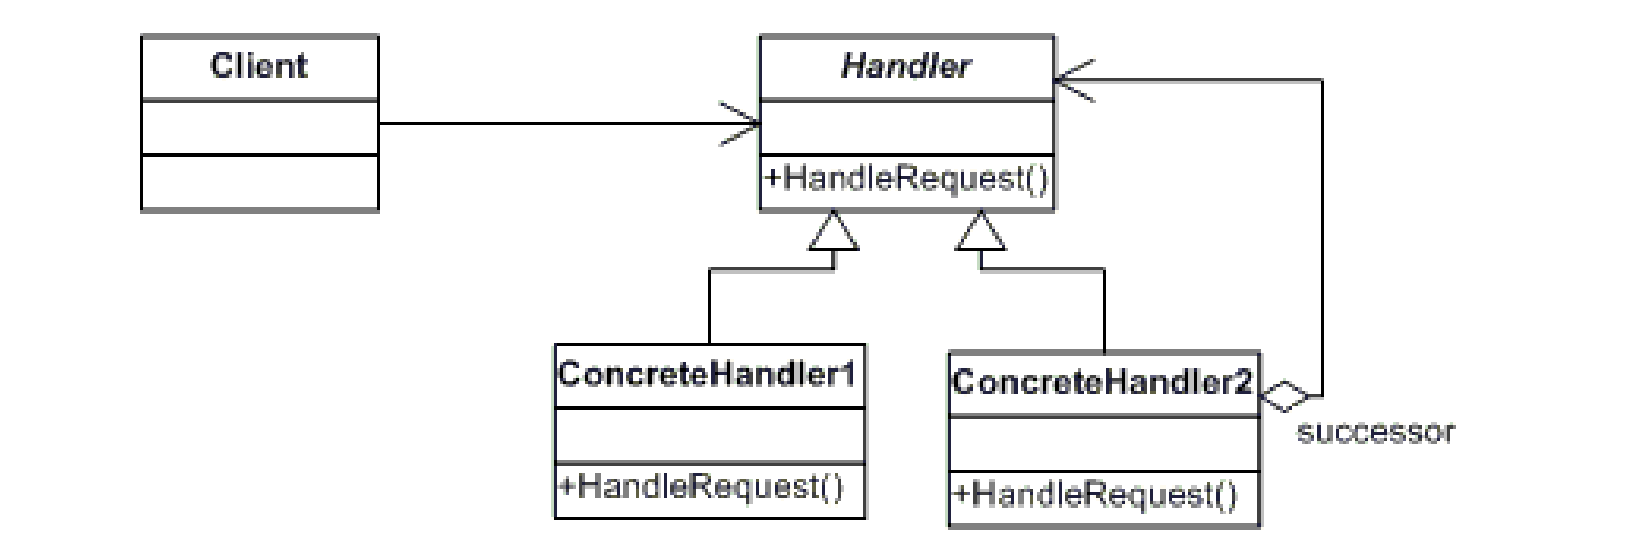
\includegraphics[width=0.5\textwidth, height=60mm]{ch-o-r.png}}
                \\

                \cmidrule(r){1-1}\cmidrule(l){2-2}
                \textbf{Iterator}
                \begin{itemize}
                    \item Umożliwienie \textbf{sekwencyjnego dostępu} do elementów kolekcji bez ujawniania jej wewnętrznej implementacji
                \end{itemize}
                &
                \raisebox{-\totalheight}{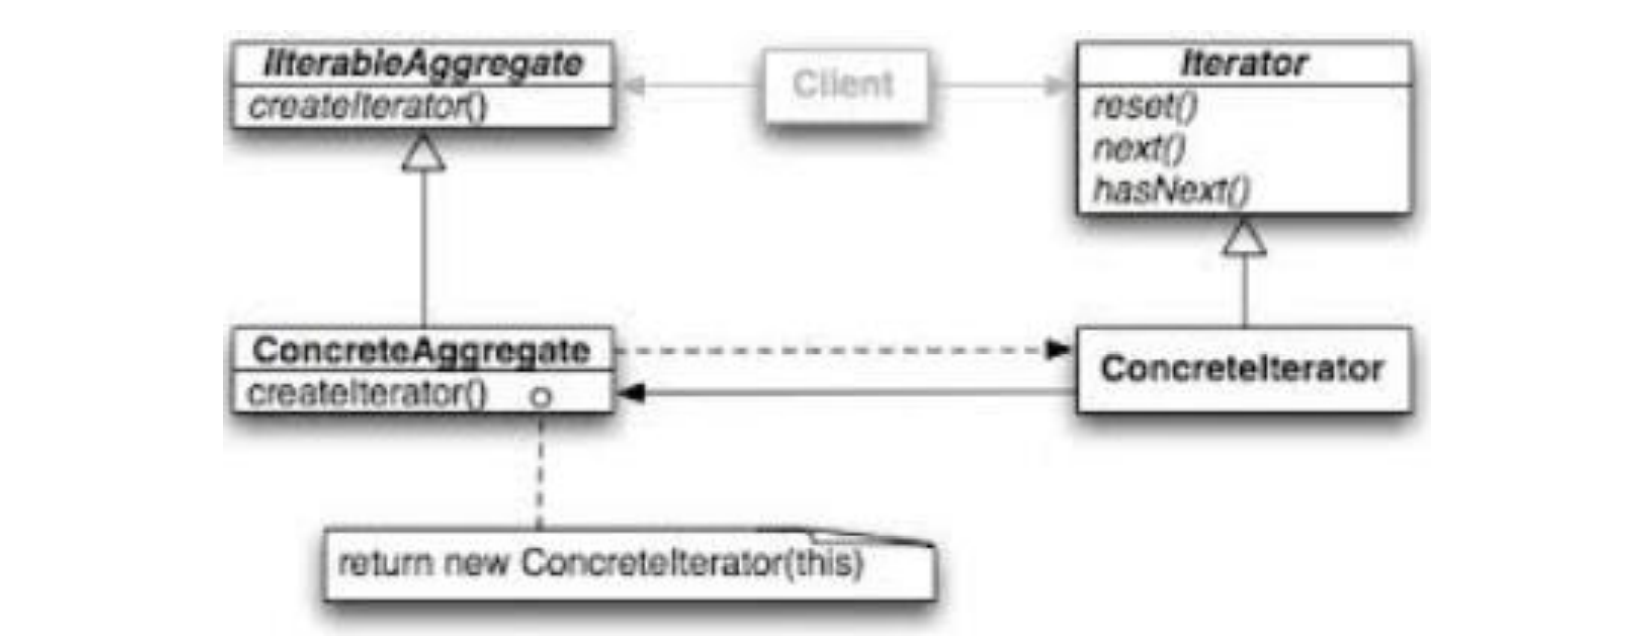
\includegraphics[width=0.5\textwidth, height=60mm]{iterator.png}}
                \\

                \bottomrule
            \end{tabular}
        \end{center}
    \end{table}


    \subsection{Implementacja wzorców projektowych}
    Implementacja to \textbf{transformowanie modelu w kod źródłowy}.

    \begin{figure}[H]
        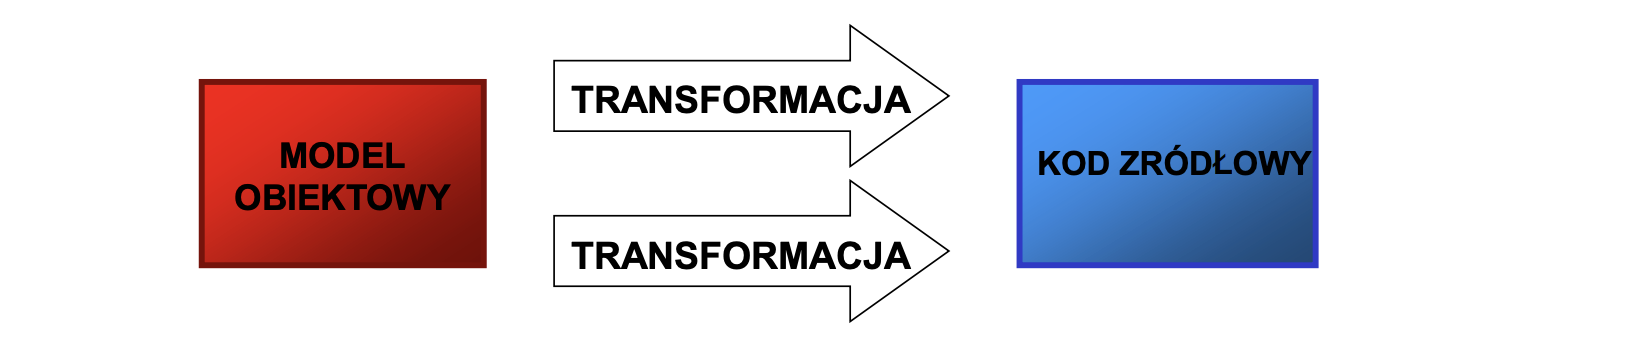
\includegraphics[width=\linewidth]{wzorce.png}
    \end{figure}

    \subsubsection{Transformacja}
    \begin{itemize}
        \item powinna dotyczyć tylko jednego, ściśle określonego kryterium,
        \item musi mieć charakter lokalny, powinna być izolowana od innych zmian,
        \item musi być poddana weryfikacji.
    \end{itemize}

    \begin{table}[H]
        \begin{center}
            \begin{tabular}{ p{8cm} p{8cm} }
                \item \textbf{Transformacja modelu}
                \begin{itemize}
                    \item ograniczona jest do samego modelu
                    \item celem jest uproszczenie lub zoptymalizowanie istniejącego modelu
                \end{itemize}
                &
                \item \textbf{Inżynieria postępująca}
                \begin{itemize}
                    \item tworzenie szablonów kodu źródłowego odpowiadającego modelowi obiektowemu
                \end{itemize}\\
            \end{tabular}
        \end{center}
    \end{table}

    \textbf{Najczęściej wykonywane} aktywności (transformacje):
    \begin{itemize}
        \item \textbf{optymalizowanie modelu} obiektowego,
        \item odwzorowywanie \textbf{skojarzeń w kolekcje},
        \item odwzorowywanie \textbf{kontraktów w wyjątki},
        \item odwzorowywanie modelu obiektowego w \textbf{schematy bazy danych}.
    \end{itemize}


    \subsubsection{Paradygmat programowania}
    \begin{itemize}
        \item wzorzec, \textbf{najogólniejszy model}, jako wzorcowy przykład,
        \item \textbf{zbiór pojęć} i teorii tworzących \textbf{podstawy} danej nauki.
    \end{itemize}


    \textbf{Podstawowe założenia}:
    \begin{itemize}
        \item \textbf{Abstrakcja} - system jako układ obiektów rozpatrywanych jako modele
        abstrakcyjnego elementu, które mogą:
        \begin{itemize}
            \item opisywać i zmieniać swój stan,
            \item komunikować się z innymi obiektami w systemie,
            \item wykonywać pewne czynności na rzecz innych obiektów bez ujawniania, w jaki sposób zaimplementowano
            dane cechy.
        \end{itemize}
        \item \textbf{Enkapsulacja}
        \begin{itemize}
            \item ukrywanie szczegółów implementacji,
            \item obiekt nie może zmieniać stanu wewnętrznego innych obiektów w nieoczekiwany sposób,
            \item tylko wewnętrzne metody obiektu są uprawnione do zmiany jego stanu,
            \item każdy typ obiektu dostarcza innym obiektom swój "interfejs", który określa dopuszczalne metody współpracy.
        \end{itemize}
        \item \textbf{Polimorfizm}
        \begin{itemize}
            \item wykazywanie różnych form działania podczas wywoływania metody w zależności od typu obiektu,
            \item referencje i kolekcje obiektów mogą dotyczyć obiektów różnego typu, a wywołanie metody dla
            referencji spowoduje zachowanie odpowiednie dla pełnego typu obiektu wywoływanego.
        \end{itemize}
        \item \textbf{Dziedziczenie}
        \begin{itemize}
            \item porządkuje i wspomaga polimorfizm i enkapsulację,
            \item umożliwia definiowanie i tworzenie specjalizowanych obiektów,
            \item dla obiektów specjalizowanych nie trzeba redefiniować całej funkcjonalności, lecz tylko tę,
            której nie mają obiekty ogólniejsze.
        \end{itemize}
    \end{itemize}

    \subsubsection{GRASP}
    General Responsibility Assignment Software Patterns - zakres odpowiedzialności.
    \begin{itemize}
        \item \textbf{Creator} - określa kiedy podany obiekt powinien tworzyć inny obiekt, tzn. B powinien tworzyć A, jeśli:
        \begin{itemize}
            \item B agreguje A,
            \item B operuje na danych obiektu A,
            \item B używa bezpośrednio A,
            \item B dostarcza informacji niezbędnej do utworzenia A
        \end{itemize}
        \item \textbf{Information Expert} - określenie danych niezbędnych do wypełnienia nowej odpowiedzialności. Programista powinien delegować ją do obiektów, które
        zawierają najwięcej informacji pozwalających ją zrealizować.
        \item \textbf{Controller} - jego zadaniem jest: odbieranie informacji od UI, wykonywanie operacji oraz zwracanie ich wyników do UI.
        Programista deleguje zadania z UI do kontrolera, a kontroler w głąb systemu.
        \item \textbf{Low Coupling} - jak największa niezależność klas.
        \item \textbf{High Cohesion} - obiekt powinien skupiać się na jednej odpowiedzialności, która powinna być jasna i nie rozmyta.
        \item \textbf{Polymorphism}
        \item \textbf{Pure Fabrication} - powstawania w systemie obiektów, które nie reprezentują
        żadnego obiektu dziedziny, a kondensują funkcje udostępniane na rzecz innych obiektów.
        \item \textbf{Indirection} - aby zapewnić low coupling często zachodzi potrzeba
        dodania mediatora w komunikacji między biektami. Jego zadaniem jest jedynie wymiana informacji
        między obiektami. Taki obiekt deleguje zadania z jednego obiektu na rzecz drugiego. Projektowanie
        systemu z użyciem mediatora wpływa na poprawę hermetyzacji elementów systemu.
        Model MVC jest dobrym tego przykładem astosowania tej zasady. Kontroler jest mediatorem, co izoluje
        interfejs użytkownika od modelu.
        \item \textbf{Protected variations} - zasada mówiąca o zakresie modyfikacji w systemie
        wymaganym przez określoną zmianę. W systemie powinno się identyfikować punkty niestabilności i
        budować interfejsy wokół tych punktów. To ograniczy zakres zmian w przypadku, gdyby
        okazało się, że podany punkt niestabilności systemu wymaga zmian.
    \end{itemize}


    \subsubsection{Metazasady}
    \begin{itemize}
        \item \textbf{Don't repeat yourself - DRY}\\
        Jedno miejsce w systemie, na pojedynczą informację, co ułatwia późniejsze zmiany.
        Inna nazwa to \textbf{Single Source Of Truth} (SSOT), każda informacja w systemie powinna być przechowywana
        dokładnie raz, bo ułatwia to jej modyfikację.
        \item \textbf{Keep it simple, stupid - KISS}\\
        W projektowaniu interfejsów powyższą zasadę można nazwać \textbf{zasadą najmniejszego zaskoczenia}, czyli
        fragment kodu powinien robić dokładnie to co ma robić. Czasem trzeba wybrać, czy dany fragment kodu
        napisać z wykorzystaniem wzorca projektowego czy prostej konstrukcji.
    \end{itemize}


\end{document}